% Copyright (c) 2015-2017, AIT Austrian Institute of Technology GmbH.
% REM All rights reserved. See file POWERFACTORY_FMU_LICENSE.txt for details.

\chapter{Examples}
\label{sec:examples}

This chapter gives examples of exporting FMUs from \pf models as described in Section~\ref{sec:export}.
All the examples use the same simple network model shown in Figure~\ref{fig:test_model}), but using different methods for defining time (trigger, \dplscript, RMS simulation).

These models are also included in the \emph{examples} folder of the \fmipp \pf Export Utility and can be used to create FMUs.
Section~\ref{sec:examples:results} provides expected simulation results as reference for testing these FMUs.

\begin{figure}[h!]
\vspace*{1em}
\centering{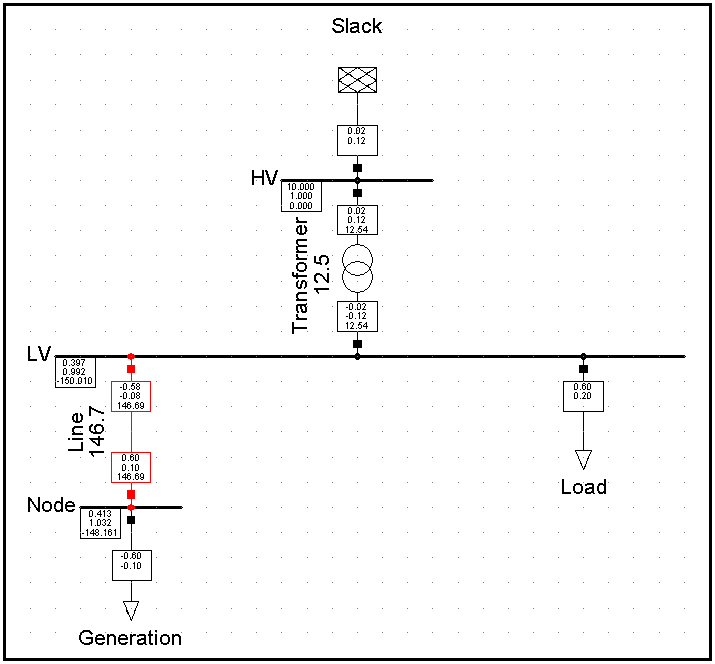
\includegraphics[width=0.74\textwidth]{test_model}}
\caption{Common power network model for example model.}
\label{fig:test_model}
\end{figure}


\section{Exporting a model using external time series and triggers}
\label{sec:examples:triggers}

An example for exporting a model using external time series and triggers can be found in subfolder \texttt{examples\symbol{92}triggers} of the installation directory.
It contains the following files:
\begin{itemize}
  \item \texttt{TestTriggers.pfd}: the \pf network model
  \item \texttt{TestTriggers-inputs.txt}: text file containing the lists of input variable names
  \item \texttt{TestTriggers-outputs.txt}: text file containing the lists of output variable names
  \item \texttt{TestTriggers-characteristics.csv}: text file containing a time series
\end{itemize}

\subsubsection*{The external time series}

In the power network model, the time series is associated with the active power (parameter \emph{plini}) of the general load named \emph{Generation}. The time series is provided in a simple text file, using semi-colons as column separators (compare to definition of \emph{File Settings} in Figure~\ref{fig:characteristics_from_file}):
\begin{Verbatim}[frame=single,commandchars=\\\{\}]
  \textcolor{black}{1;-0.5}
  \textcolor{black}{2;-0.4}
  \textcolor{black}{3;-0.3}
  \textcolor{black}{4;-0.2}
  \textcolor{black}{5;-0.1}
\end{Verbatim}

\subsubsection*{Executing the export script}

To export the network model as FMU, issue the following command in the command prompt window (directly from the directory containing the files):
\begin{verbatim}
python.exe ..\..\powerfactory_fmu_create.py -m PFTestTriggers \
  -i TestTriggers-inputs.txt -o TestTriggers-outputs.txt \
  -p TestTriggers.pfd -t Trigger:60 TestTriggers-characteristics.csv \
  ElmLod.Load.plini=0.6
\end{verbatim}
Some comments:
\begin{itemize}
  \item This command defines \emph{PFTestTriggers} as FMI model identifier.
  Hence, the resulting FMU is called \texttt{PFTestTriggers.fmu}.
  \item The command specifies one trigger called \texttt{Trigger}, with a scale of 60.
  This means that at master simulation time $T$ (in seconds), the associated characteristic in \pf will produce the time series value associated to $T/60$.
  For instance, at simulation time $T=180\,$s, the characteristic will produce the value $-0.3$ (compare with definition of time series above).
  \item The file containing the time series is explicitly declared as additional input file.
  In the \pf model, this file should be referred to directly by name, without a leading path (compare to Figure~\ref{fig:characteristics_from_file}).
  \item The active power (parameter name \emph{plini}) of the general load called \emph{Load} is initialized with the value $0.6$.
\end{itemize}

\newpage

\section{Exporting a model using a \dplscript}
\label{sec:examples:dplscript}

An example for exporting a model using a \dplscript can be found in subfolder  \texttt{examples\symbol{92}dplscript} of the installation directory.
It contains the following files:
\begin{itemize}
  \item \texttt{TestDPLScript.pfd}: the \pf network model
  \item \texttt{TestDPLScript-inputs.txt}: text file containing the lists of input variable names
  \item \texttt{TestDPLScript-outputs.txt}: text file containing the lists of output variable names
\end{itemize}

\subsubsection*{Associating a characteristic with the \dplscript}

In the power network model, a 1-dimensional characteristic is associated with the active power (parameter \emph{plini}) of the general load named \emph{Generation}.
Also, the \pf model contains a \dplscript that takes the second of the year as input to set the simulation time (compare with the \dplscript shown in Section~\ref{sec:export:create_model_dplscript}).

\subsubsection*{Executing the export script}

To export the network model as FMU, issue the following command in the command prompt window (directly from the directory  containing the files):
\begin{verbatim}
python.exe ..\..\powerfactory_fmu_create.py -m PFTestDPLScript \
  -i TestDPLScript-inputs.txt -o TestDPLScript-outputs.txt \
  -p TestDPLScript.pfd -s SetTime:1:0 ElmLod.Load.plini=0.6
\end{verbatim}
Some comments:
\begin{itemize}
  \item This command defines \texttt{PFTestDPLScript} as FMI model identifier.
  Hence, the resulting FMU is called \texttt{PFTestDPLScript.fmu}.
  \item The command specifies the name of the \dplscript as \emph{SetTime}, with a scale of 1 and an offset of 0.
  This means that at master simulation time $T$ (in seconds), the associated \dplscript will be called with an input argument value of $T/1 + 0$.
  Since in this case the \dplscript expects the second of the year as input argument, simulation time 0 coincides with the beginning of the year.
  \item The active power (parameter name \emph{plini}) of the general load called \emph{Load} is initialized with the value $0.6$.
\end{itemize}


\newpage


\section{Exporting a model for RMS simulation}
\label{sec:examples:rmssim}

An example for exporting a model for RMS simulation can be found in subfolder \texttt{examples\symbol{92}rms} of the installation directory.
It contains the following files:
\begin{itemize}
  \item \texttt{TestRMS.pfd}: the \pf model
  \item \texttt{TestRMS-inputs.txt}: text file containing the lists of input variable names
  \item \texttt{TestRMS-outputs.txt}: text file containing the lists of output variable names
\end{itemize}

\subsubsection*{Model Structure}

The \pf model contains in subfolder \emph{Library} $\to$ \emph{User Defined Models} the following objects (see Figure~\ref{fig:example_rms_model_browser}):
\begin{itemize}
  \item \emph{ControllerForTwoLoads}: This \dslmodel (type \texttt{BlkDef}) defines two output signals, \emph{outPext1} and \emph{outPext2}, and two parameters, \emph{Pext1} and \emph{outPext2}, see Figure~\ref{fig:controller_for_two_loads}.
  In this simple example, the output signals are a direct "feedthrough" of the values of the parameters, as defined by the model's DSL equation (see Figure~\ref{fig:controller_for_two_loads_equ}).
  \item \emph{FMIAdapter}: block-definition of compiled \dslmodel FMIAdapter (see Section~\ref{sec:export:create_model_rms})
  \item \emph{FMIAdapterConfig}: composite model frame (type \texttt{BlkDef}) defining slots for the FMIAdapter, the controller and two loads as well as the connections between the controller and the loads, see Figure\ref{fig:fmiadapterconfig_composite_frame_2}
\end{itemize}

Furthermore, Figure~\ref{fig:example_rms_model_browser} shows that subfolder \emph{Network Model} $\to$ \emph{Network Data} $\to$ \emph{Grid} contains a composite model called \emph{FMIAdapterImplementation} (type \texttt{ElmComp}, see Figure~\ref{fig:fmiadapterconfig_composite_model}), which implements the composite frame FMIAdapterConfig.
It also contains common models (type \texttt{ElmDsl}) that implement the {\dslmodel}s defining the FMIAdapter and the ControllerForTwoLoads.
See for example Figure~\ref{fig:controllerinstance}, which shows the definition of common model \emph{ControllerInstance}.

\begin{figure}[h!]
%\vspace*{2em}
\centering{\fbox{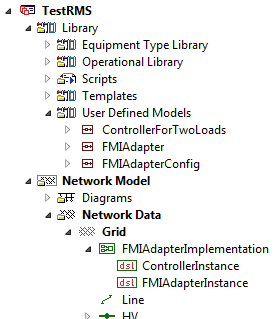
\includegraphics[width=0.45\textwidth]{example_rms_model_browser}}}
\caption{View of the data manager for \pf model TestRMS.}
\label{fig:example_rms_model_browser}
\end{figure}

\begin{figure}[h!]
\vspace*{1em}
\centering{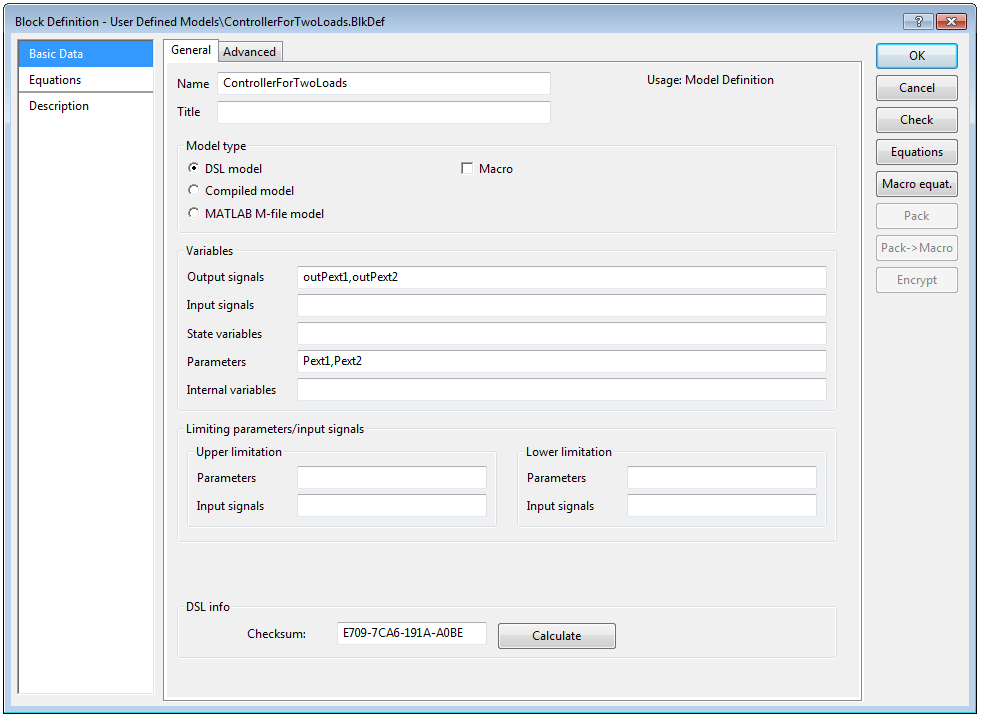
\includegraphics[width=0.98\textwidth]{controller_for_two_loads}}
\caption{Model definition of controller, including definition of output signals and parameters.}
\label{fig:controller_for_two_loads}
\end{figure}

\begin{figure}[h!]
\vspace*{2em}
\begin{Verbatim}[frame=single,commandchars=\\\{\}]
  \codeHighlightGreen{! Initial conditions for output signals.}
  \codeHighlightBlue{inc}\textcolor{black}{(outPext1) = Pext1}
  \codeHighlightBlue{inc}\textcolor{black}{(outPext2) = Pext2}

  \codeHighlightGreen{! Associate output signals with model parameters.}
  \textcolor{black}{outPext1 = Pext1}
  \textcolor{black}{outPext2 = Pext2}
\end{Verbatim}
\vspace*{-2ex}
\caption{DSL equations of controller.}
\label{fig:controller_for_two_loads_equ}
\end{figure}


\begin{figure}[h!]
\vspace*{1em}
\centering{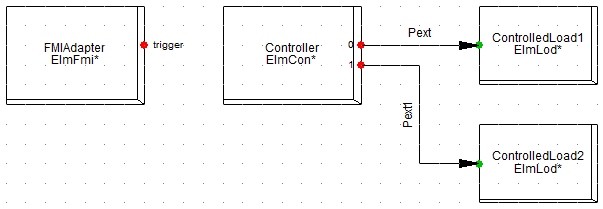
\includegraphics[width=0.7\textwidth]{fmiadapterconfig_composite_frame}}
\caption{Composite frame including \dslmodel FMIAdapter and a controller connected to two loads.}
\label{fig:fmiadapterconfig_composite_frame_2}
\end{figure}

\clearpage

\subsubsection*{Sending simulation events}

File \texttt{TestRMS-inputs.txt} contains the definition of two input variables:
\begin{Verbatim}[frame=single,commandchars=\\\{\}]
  \textcolor{black}{EvtParam.Controller.Pext1}
  \textcolor{black}{EvtParam.Controller.Pext2}
\end{Verbatim}
According to the naming convention (see Section~\ref{sec:naming_convention:sim_evt}), these two input variables correspond to simulation events.

When a new value is set for one of these two input variables at a synchronization point during the simulation, a simulation event is immediately issued in \pf.
The instance of the FMIAdapter model (in this example common model FMIAdapterInstance) will send the event to the corresponding slot of the composite frame that it belongs to (in this example slot Controller of composite frame FMIAdapterConfig).
Then the parameters of the model associated to this slot will be set to the new value (in this example parameters Pext1 or Pext2 of \dslmodel ControllerForTwoLoads).
Depending on the settings of \pf (mainly the integrator step size), the event will be executed within a short delay as soon as the next simulation step is started.

\begin{figure}[h!]
\vspace*{2em}
\centering{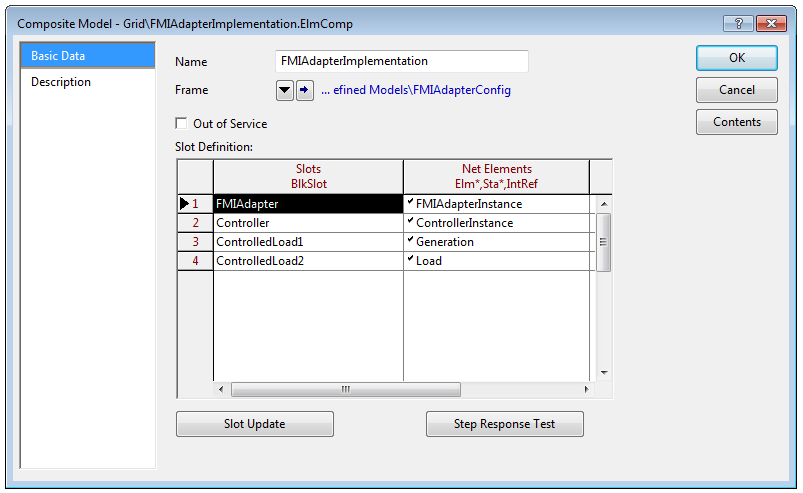
\includegraphics[width=0.98\textwidth]{fmiadapterconfig_composite_model}}
\caption{Definition of composite model FMIAdapterImplementation, implementing the composite frame (FMIAdapterConfig) and assigning the slots to common models and network elements.}
\label{fig:fmiadapterconfig_composite_model}
\end{figure}

\newpage

\begin{figure}[h!]
\vspace*{2em}
\centering{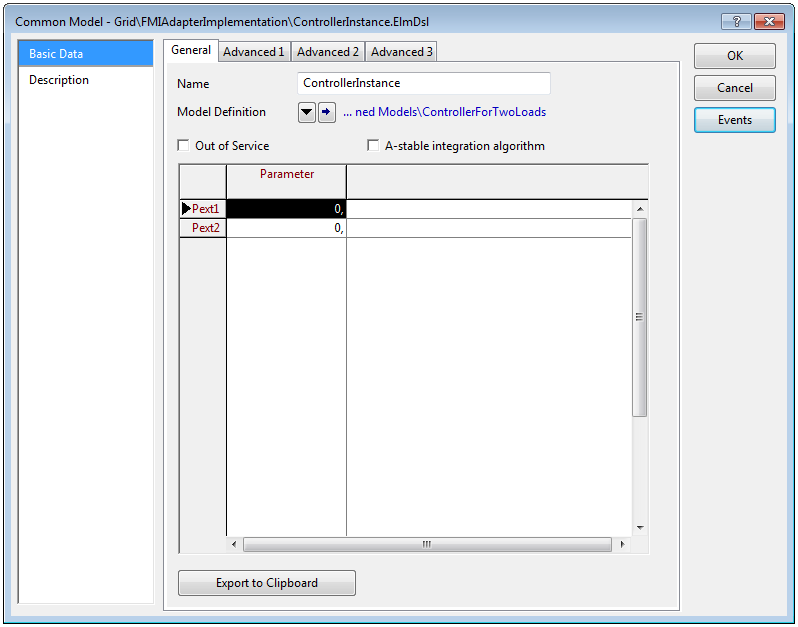
\includegraphics[width=0.98\textwidth]{controllerinstance}}
\caption{Definition of common model ControllerInstance, implementing \dslmodel ControllerForTwoLoads for common model FMIAdapterImplementation.}
\label{fig:controllerinstance}
\end{figure}

\subsubsection*{Executing the export script}

To export the network model as FMU, issue the following command in the command prompt window (directly from the directory  containing the files):
\begin{verbatim}
python.exe ..\..\powerfactory_fmu_create.py -m PFTestRMS \
  -i TestRMS-inputs.txt -o TestRMS-outputs.txt \
  -p TestRMS.pfd -r 1 ElmLod.Load.plini=0.6
\end{verbatim}
Some comments:
\begin{itemize}
  \item This command defines \emph{PFTestRMS} as FMI model identifier.
  Hence, the resulting FMU is called \texttt{PFTestRMS.fmu}.
  \item The command specifies an integrator step size of 1~second for the RMS simulation.
  \item The active power (parameter name \emph{plini}) of the general load called \emph{Load} is initialized with the value $0.6$.
\end{itemize}


\newpage

\section{Reference results}
\label{sec:examples:results}

The examples above are included in the \emph{examples} folder of the \fmipp \pf Export Utility and can be used to create FMUs for testing.
This section provides expected simulation results as reference for testing the created FMUs.

\subsection{Results for using the model with an external time series and a trigger}
\label{sec:examples:results_trigger}

When properly exported and used within a co-simulation framework (without any further inputs), the results in Table~\ref{tab:examples:trigger_outputs} should be observed for output variable \texttt{ElmTerm.Node.m:u} (FMI value reference 1001):

\begin{table}[h!]
\centering{\begin{tabular}{|c|c|}
    \hline 
    simulation time & \texttt{ElmTerm.Node.m:u} \\ 
    \hline \hline 
    1~min & 1.026309 \\ \hline 
    2~min & 1.020366 \\ \hline 
    3~min & 1.014217 \\ \hline 
    4~min & 1.007850 \\ \hline 
    5~min & 1.001254 \\ \hline 
  \end{tabular}}
\caption{Expected outputs from model with an external time series and a trigger.}
\label{tab:examples:trigger_outputs}
\end{table}



\subsection{Results for using the model with a \dplscript}
\label{sec:examples:results_dplscript}

When properly exported and used within a co-simulation framework (without any further inputs), the same results as for the model with an external time series and a trigger should be observed (see Section~\ref{sec:examples:results_trigger} above).


\subsection{Results for using the model for RMS simulation}
\label{sec:examples:results_rms}

When properly exported and used within a co-simulation framework, the inputs given in Table~\ref{tab:examples:rms_inputs} should be applied.
Table~\ref{tab:examples:rms_outputs} lists the results that should be observed.
Please note that the synchronization points for setting inputs are not the same as for reading outputs.


\begin{table}[h!]
\centering{\begin{tabular}{|c|c|c|}
    \hline 
    simulation time & \texttt{EvtParam.Controller.Pext1} & \texttt{EvtParam.Controller.Pext2} \\ 
    \hline \hline 
    0~s & -1.0 & 2.0 \\ \hline 
    60~s & -0.5 & 0.5 \\ \hline 
    120~s & -1.0 & 1.0 \\ \hline 
    180~s & -1.5 & 1.5 \\ \hline 
    240~s & -2.0 & 2.0 \\ \hline 
\end{tabular}}
\caption{Inputs for RMS simulation.}
\label{tab:examples:rms_inputs}

\vspace*{2ex}

\centering{\begin{tabular}{|c|c|c|}
    \hline 
    simulation time & \texttt{ElmTr2.Transformer.m:P:buslv} & \texttt{ElmLod.Generation.m:I1:bus1} \\ 
    \hline \hline 
    30~s & -0.895882 & 1.489078 \\ \hline 
    90~s & 0.014029 & 0.732799 \\ \hline 
    150~s & 0.054946 & 1.503625 \\ \hline 
    210~s & 0.119682 & 2.307266 \\ \hline 
    270~s & 0.203200 & 3.136092 \\ \hline
\end{tabular}}
\caption{Expected outputs from RMS simulation.}
\label{tab:examples:rms_outputs}
\end{table}

